% TEX compiler = latexmk
\documentclass[12pt]{article}

\usepackage{graphicx}
\usepackage{amsmath}
\usepackage{fancyhdr}
\usepackage{geometry}
\usepackage{circuitikz}
\usepackage{subfigure}
\usepackage{caption}
\usepackage{karnaugh-map}
\usepackage{bm}
\usepackage{float}

\geometry{letterpaper, margin=1in}
\graphicspath{ {../images/} }

% Header and Footer
\pagestyle{fancy}
\fancyhf{}
\fancyhead[L]{CSE 2301 - Lab 05: Two's Complement and Adders}
\fancyhead[R]{\thepage}
\setlength{\headheight}{15pt}

\author{Arturo Salinas-Aguayo}
\title{Lab 05: Two's Complement and Adders}
% theorem set
\newtheorem{example}{Example}
% Example block environment
\newenvironment{examp}
{\vspace{0.5cm}
\hrule
\begin{example}}
{\hrule
\vspace{0.5cm}
\end{example}}

\begin{document}
\newcommand{\closure}[2][3]{%
	{}\mkern#1mu\overline{\mkern-#1mu#2}}
\newcommand\ncoverline[1]{\mkern1mu\overline{\mkern-1mu#1\mkern-1mu}\mkern1mu}
% Title Page
\begin{titlepage}
	\centering
	\vspace*{3cm}
	\huge\textbf{Lab 05: Two's Complement and Adders}\\
	\vspace{5cm}
	\Large\textbf{Arturo Salinas-Aguayo}\\
	\normalsize
	CSE 2301: Principles and Practice of Digital Logic Design\\
	Dr. Mohammad Khan, Section 003L-1248\\
	Electrical and Computer Engineering Department
	\vfill
	
\includegraphics[scale=0.1]{uconnlogo}\\
	College of Engineering, University of Connecticut\\
	\scriptsize{Coded in \LaTeX}
	\vspace*{1cm}
\end{titlepage}
\section*{Theory}
\subsection*{What is 2’s Complement Anyway?}
Two’s Complement is a method of encoding signed integers in binary form, where the most significant bit indicates the sign (0 for positive, 1 for negative). The remaining bits represent the magnitude of the number. To convert a positive number to its Two’s Complement negative equivalent, you invert all the bits and add 1 to the result.

We use Two’s Complement because it simplifies arithmetic operations like addition and subtraction in digital circuits. Unlike signed-magnitude representation, Two’s Complement eliminates the need for separate circuitry to handle negative numbers. This makes it efficient and less prone to error in binary arithmetic operations.
\subsubsection*{Why the Cout Pin Overflow is Misleading}
When adding two numbers in Two’s Complement, the Cout pin in a full-adder indicates a carry-out. However, this can be misleading when detecting overflow, especially in signed arithmetic. For example, adding -3 and +5 in Two’s Complement could result in a carry-out even though no overflow occurred from a signed arithmetic perspective. Instead of relying on the Cout pin, overflow detection should focus on cases where the signs of the two operands are the same but the result has a different sign.

In my circuit for Part 3, I detected overflow by using combinational logic to identify when two positive numbers resulted in a negative number, or two negative numbers resulted in a positive number.

This reinforces the importance of understanding the use of the different pins in the full-adder and the limitations of the Cout pin in detecting overflow in signed arithmetic. For example, the adder can also be used to subtract by using the Two's Complement of the number to be subtracted. This is a key concept in the design of Arithmetic Logic Units (ALUs) in processors.
\begin{examp}
	\textbf{Labeled Chip and Pin Symbols.}\newline
	Figure 1 and Figure 2 are the labeled symbols for both the 2’s Complement Converter and the Overflow Detector, respectively.

	All of the pins and chips are labeled according to the following notation: \(UX\) where \(X\) is a number to denote the chip, followed by a dash and lowercase letter to denote the gate on the chip. This is common notation on electrical diagrams.

	The key for these is on the bottom right of each figure.
	\begin{figure}[H]
		\center{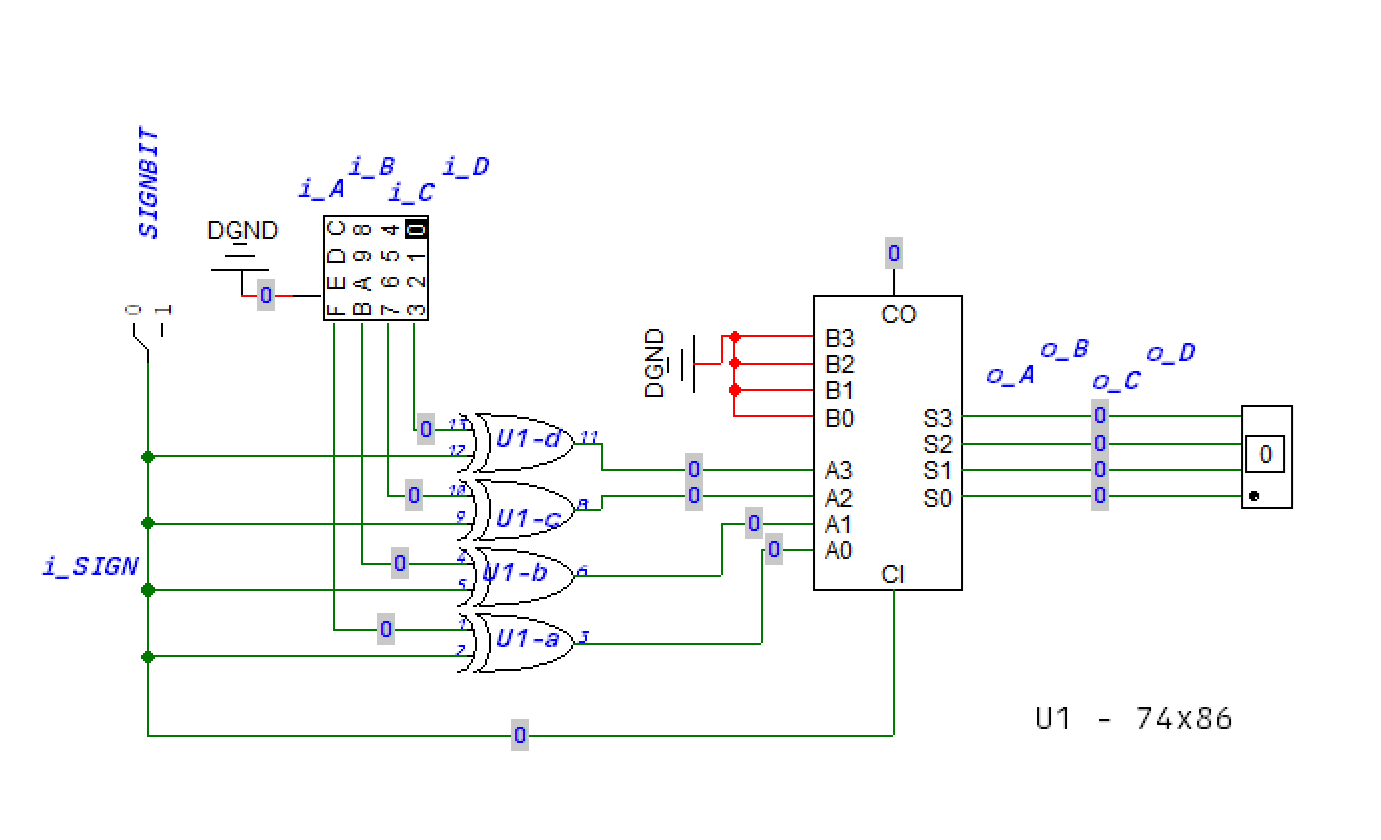
\includegraphics[scale=.75]{twoscompliment.png}}
		\caption{2's Complement Converter}
	\end{figure}

	\begin{figure}[H]
		\center{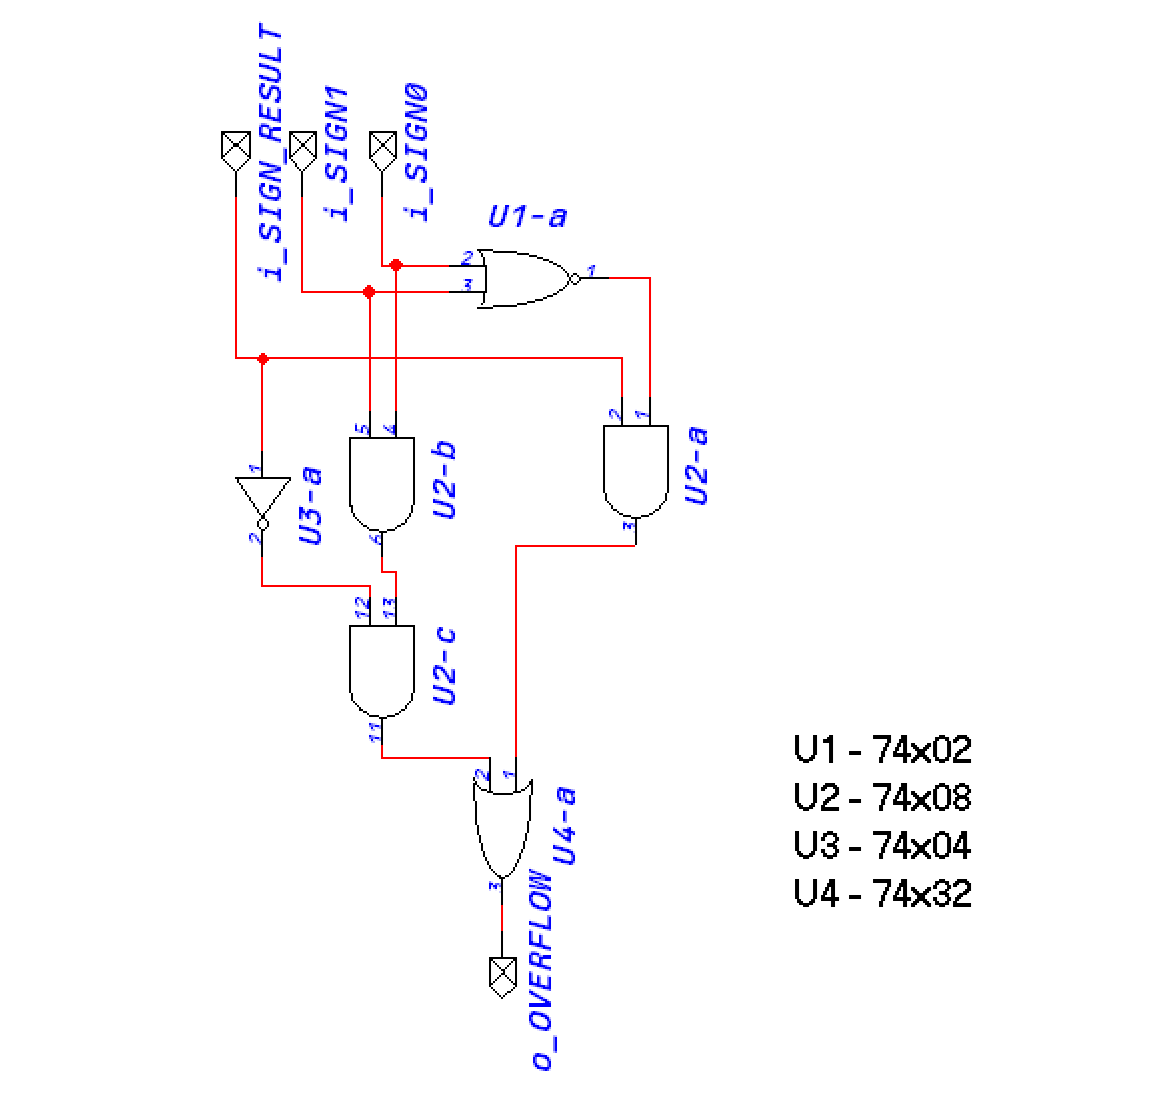
\includegraphics[scale=.65]{overflow.png}}
		\caption{Overflow Detector}
	\end{figure}
\end{examp}

\begin{examp}
	\textbf{Test Cases} \\
	Below is a table of eight test cases, listing the inputs, and showing the magnitude, sign, and overflow of the outputs.
	Recall that "Sign of Result" is 1 if the result is negative, and 0 if the result is positive. "Overflow" is 1 if an overflow occurred, and 0 if no overflow occurred.
	\begin{table}[H]
		\centering
		\begin{tabular}{|c|c|c|c|c|}
			\hline
			\textbf{Input A} & \textbf{Input B} & \textbf{Hex Output} & \textbf{Sign of Result} & \textbf{Overflow} \\
			\hline
			4                & 6                & 6                   & 1                       & 1                 \\
			C                & A                & 6                   & 0                       & 0                 \\
			3                & D                & 0                   & 0                       & 0                 \\
			7                & 7                & 2                   & 1                       & 1                 \\
			-7               & 8                & 1                   & 0                       & 0                 \\
			-6               & A                & 4                   & 0                       & 0                 \\
			-4               & -4               & 8                   & 1                       & 0                 \\
			\hline
		\end{tabular}
		\caption{Test Cases Table}
	\end{table}
	\begin{figure}[H]
		\centering
		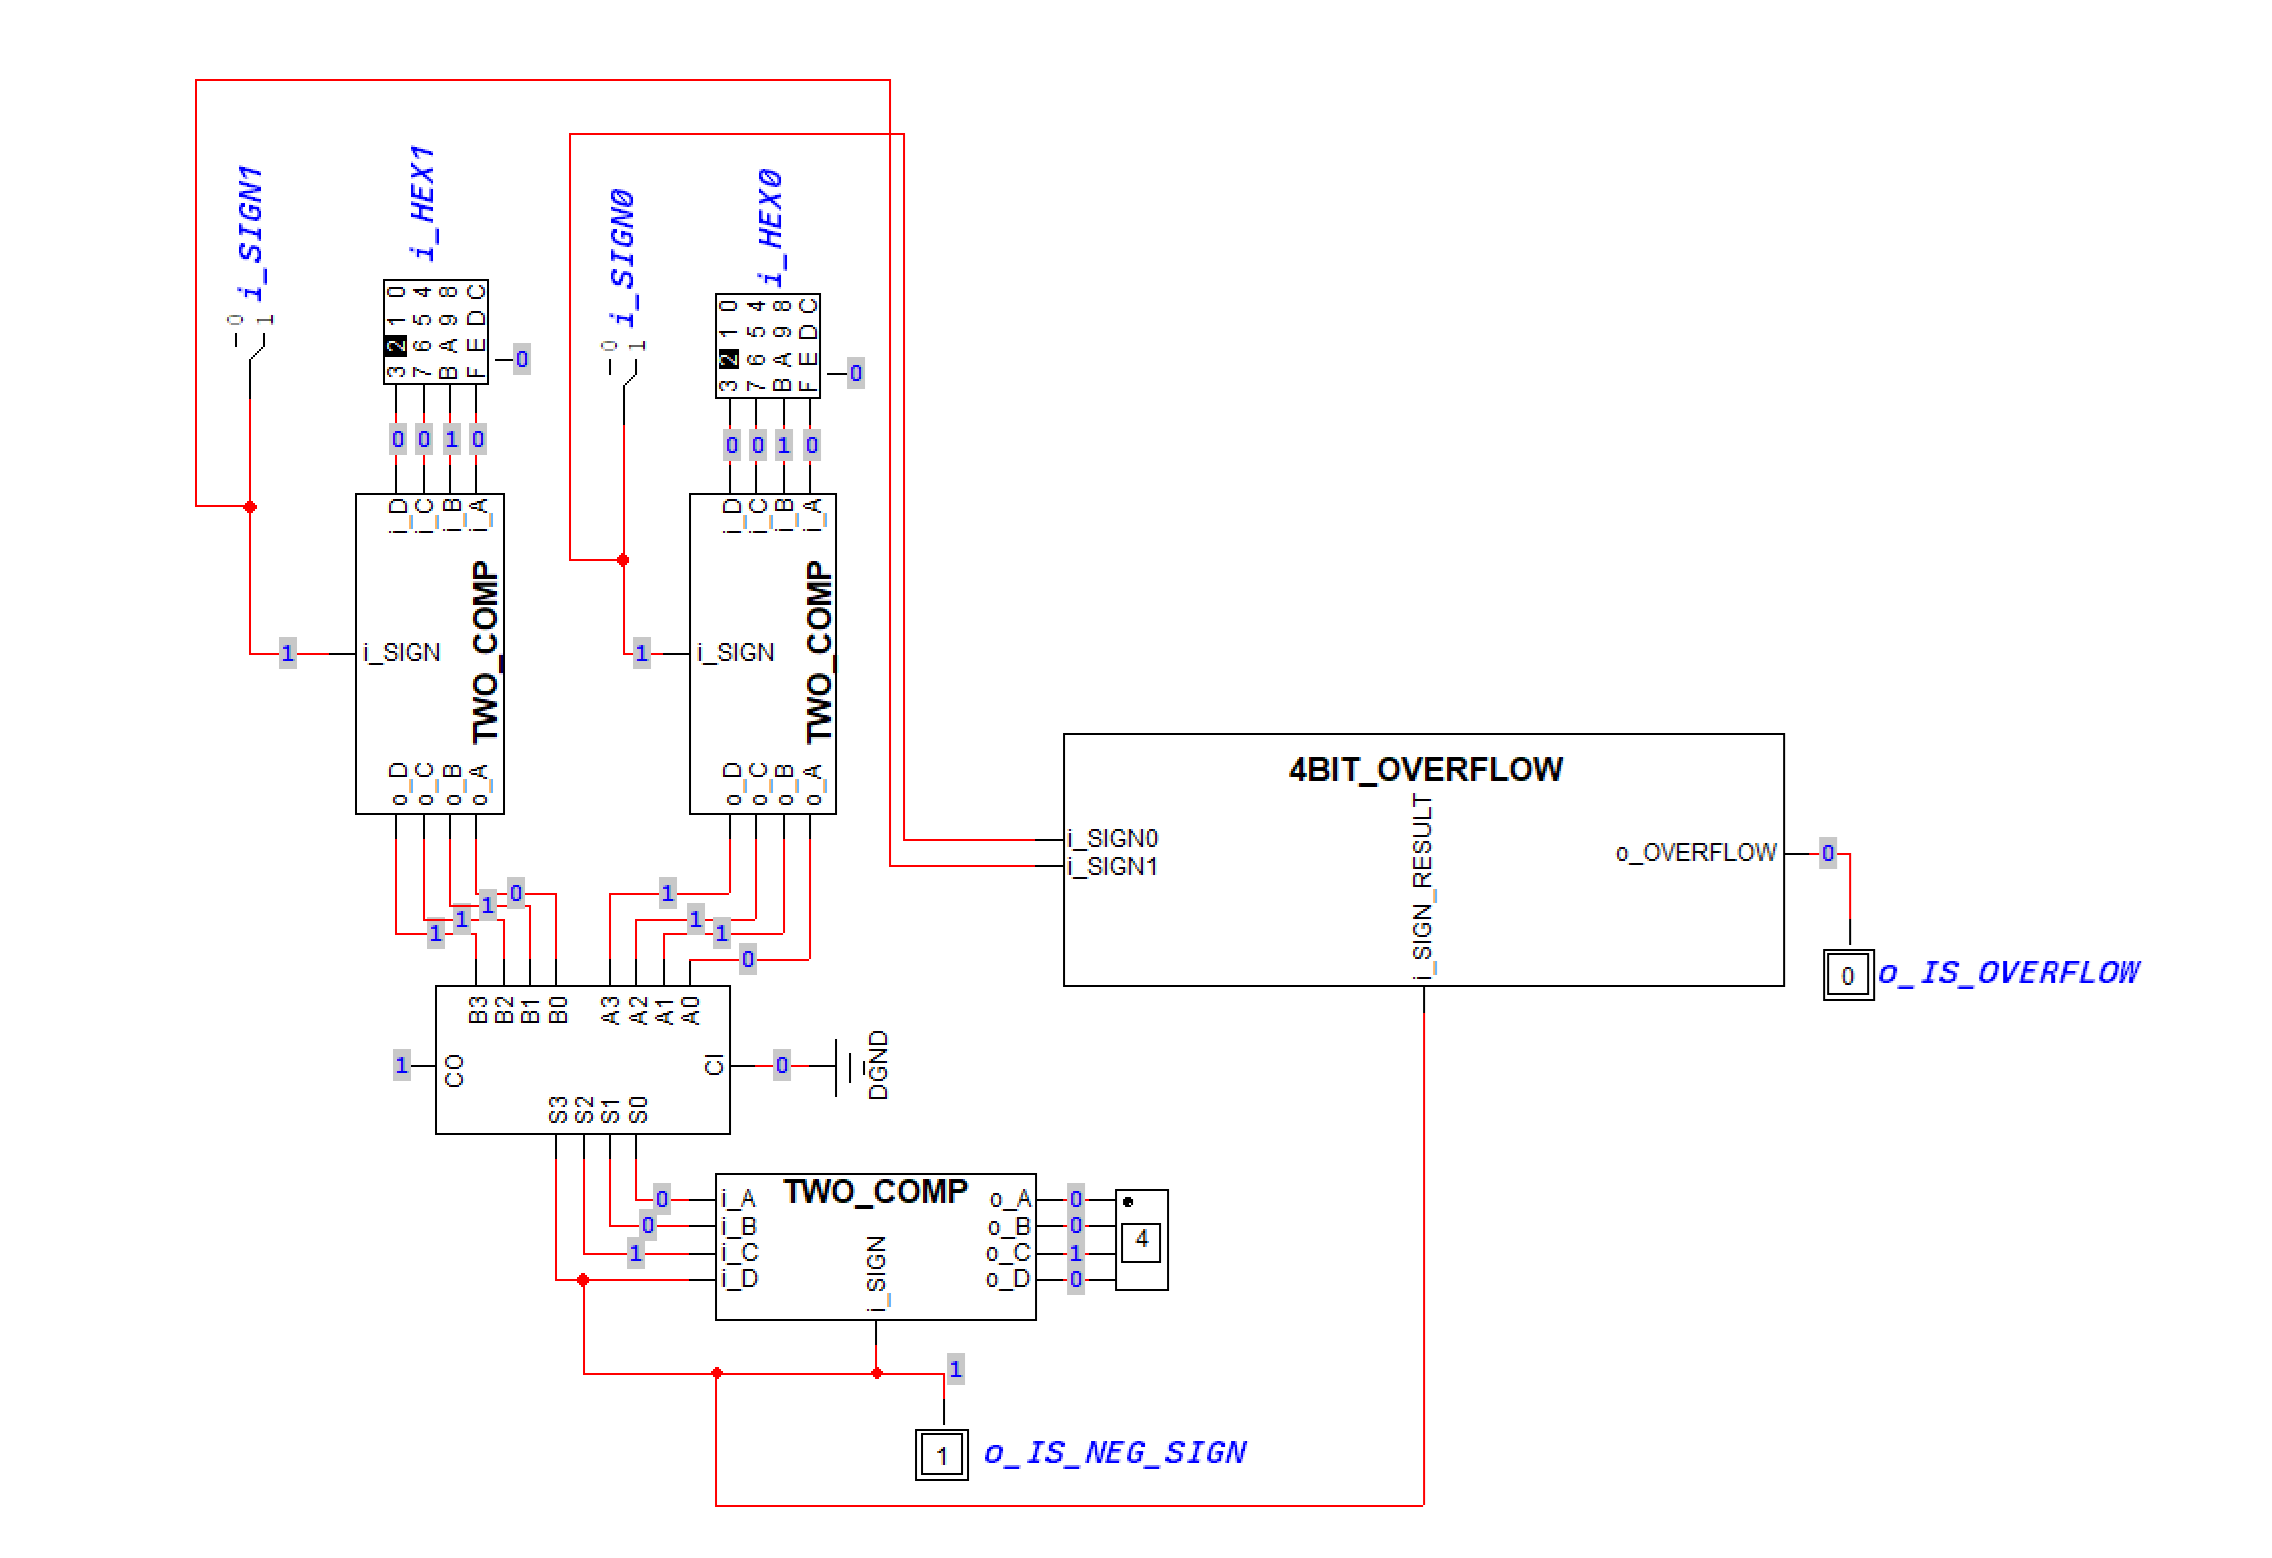
\includegraphics[scale=.5]{overflower.png}
		\caption{Overflow Detector Circuit}
	\end{figure}
	\subsubsection*{Test Case Selection}
	\textnormal{
		The test cases were selected to cover a range of inputs, including both positive and negative numbers, as well as cases with and without overflow. Since exhaustive testing is not feasible, I focused on cases that would trigger different logic paths, such as adding two large positive numbers, two large negative numbers, and combinations that should produce no overflow. Essentially, if I expected a negative and got a positive number, I knew something was awry and overflowed.}\newline
\end{examp}
\subsection*{Discussion}
This lab helped reinforce my understanding of Two’s Complement arithmetic and the importance of accurate overflow detection in digital circuits. The process of creating reusable symbols in LogicWorks was particularly valuable, as it streamlined the development of complex circuits. Detecting overflow through combinational logic instead of relying on the Cout pin was a key takeaway, as it highlighted the differences between binary and signed arithmetic. Overall, this lab improved my circuit design skills and my ability to implement Two’s Complement in a practical setting.

There were some difficulties in learning the software, but after spending some time reading the reference material (which is sadly incomplete due to the age of the software), some great strides were made in implementing combinational circuitry. Looking forward to the VHDL chapter, I changed my inputs to better make sense when dealing with behaviorial or RTL descriptions of these circuits in the future. That alongisde the ability to specify pins brings the software closer to the hardware implementation.

This also sets us up for the next lab which is a basic ALU implementation, by using the overflow detector and the 2's complement converter, we can now implement the adder and the subtractor in the ALU.
\begin{examp}
	\textnormal
	\textbf{Timing Diagram for a Combinational Circuit.}
	\begin{enumerate}
		\item  \textbf{Initial State (before \(t = 5 \, \text{ns}\)):}
		      \begin{itemize}
			      \item Inputs are stable: \(A = 1\), \(B = 1\), \(C = 0\), \(D = 1\).
			      \item  Outputs are stable based on these inputs.
		      \end{itemize}
		\item \textbf{At \(\mathbf{t = 5 \, \text{ns}}\):}
		      \begin{itemize}
			      \item \(A\) changes from 1 to 0.
			      \item  The change in \(A\) propagates through the circuit, starting with the inverters and continuing to the AND/OR gates.
		      \end{itemize}
		\item \textbf{Inverter Delay:}
		      \begin{itemize}
			      \item \(\closure{A}\), the inverted form of \(A\), takes 5 ns to reflect the change, becoming 1 at \(t = 10 \, \text{ns}\).
		      \end{itemize}
		\item \textbf{AND/OR Gate Delay:}
		      \begin{itemize}
			      \item Gates dependent on \(\closure{A}\) or \(A\) (such as signals \(H\), \(E\), and \(F\)) will take an additional 10 ns to reflect the change. Thus, the outputs of these gates begin to change at \(t = 15 \, \text{ns}\).
		      \end{itemize}
	\end{enumerate}
	- \textbf{Transient Behavior:} A transient (or glitch) occurs when the output temporarily toggles due to the varying delays in the circuit.
	\newline
	- \textbf{Transients Observed:} The timing diagram shows transients for signals \(H\), \(E\), \(F\), and \(G\) between \(t = 5 \, \text{ns}\) and \(t = 15 \, \text{ns}\), caused by the delayed propagation of the input changes through the inverters and gates.
	\begin{figure}[H]
		\centering
		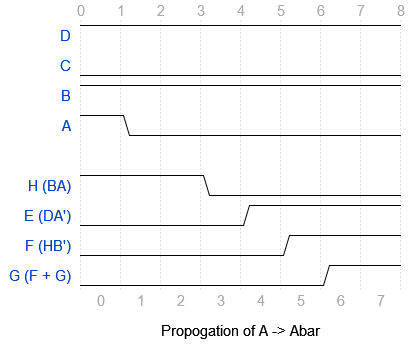
\includegraphics[scale=.45]{examp051.png}
		\caption{Timing Diagram}
	\end{figure}

\end{examp}
\begin{examp}
\textbf{Static 1-Hazard Elimination.} \\
Consider the Boolean function \( F = (\closure{A}\closure{B}) + BD \), which is a two-level AND-OR combinational circuit. A static 1-hazard occurs if, in response to a single input change, the output momentarily goes to 0 when it should remain constant at 1. To eliminate this hazard, we follow these steps.

\subsubsection*{Identify the Static 1-Hazard.}
The static 1-hazard in the circuit can be detected by examining adjacent minterms on a Karnaugh map (K-map) for the function \( F \). Adjacent 1's that are not covered by a single loop indicate the presence of a hazard. In this case, the minterms \(\closure{A}\closure{B}\) and \( BD \) do not cover all the transitions between the states where the output should remain constant.

The K-map for the function \(F = \sum m(0,1,3,7)\) is shown below. The red and green implicant  circles represent the two groups of minterms that cover the function. The static 1-hazard occurs between the minterms \( (\closure{A}\closure{B}) \) and \( BD \). The yellow implicant is the missing minterm that causes the hazard. To fix the static-1 hazard, we need to add this minterm to the expression.
\begin{center}
\begin{karnaugh-map}(label=corner)[2][4][1][$D$][$A$][$B$]
\minterms{0,1,3,7}
\implicant{0}{1}
\implicant{3}{7}
\implicant{1}{3} % oh no static-1 hazard!!!!
\autoterms[0]
\end{karnaugh-map}
\end{center}
\vspace{5mm}
\subsubsection*{Adding a Minterm to Eliminate the Hazard.}

By analyzing the K-map, we see that the yellow implicant circle overlaps with the other two circles.  that the minterm \( AB \) is missing. Adding this minterm ensures that the circuit transitions smoothly without introducing any glitches. The new expression becomes:
\[
	F = (\closure{A}\closure{B})  + BD + AB
\]
This eliminates the static 1-hazard by covering the transition between \((\closure{A}\closure{B})\) and \( BD \).
\end{examp}


\end{document}
% vim: set spell spelllang=en_us expandtab tabstop=4 shiftwidth=4 softtabstop=4:
